\chapter{Background and Related Work}
\label{chap:background}

This chapter contains the literature survey and the background for the thesis. Background on various concepts used in the thesis alongwith numerous related studies, especially on Twitter data are then discussed.


\section{Summarization}

Summarization is the task of condensing the original text document while retaining as much of the important information as possible. Other goals include readability of the generated summary and coherence. The two main approaches for automatic text summarization are \textit{extractive} and \textit{abstractive} summarization. Extractive summarization uses the technique of extract and rearrange. \cite{nenkova2012survey} describe the components in extractive summarization techniques as building an internal representation of the important parts of the text, ranking these in the order of importance/time etc and then selecting a suitable list of these sentences to eventually form the summary. In phrase-level summarization, smoothing techniques may be used to generate readable texts. Sentence-level summarization techniques tend do be inherently more cohesive since sentences are directly picked out, however, sentence compression techniques can be used to reduce the size of the summaries. Even after using smoothing techniques to generate readable text, the summaries tend to be incoherent and hard to read. \figref{fig:extractive} shows an example of extractive summarization where a couple of sentences from the article have been picked to show in the the thumbnail for an article.

\begin{figure}[!htbp]
\centering
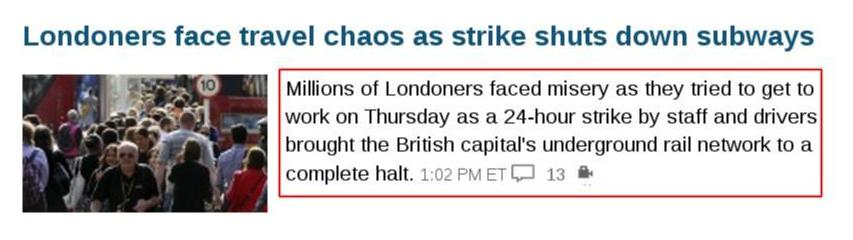
\includegraphics[width=\textwidth, height=4.5cm]{extractive}
\caption{Example of extractive summarization.}
\label{fig:extractive}
\end{figure}


The second approach is that of abstractive summarization. This is a text-to-text generation approach that aims at keeping the content or meaning of the text the same while condensing the text or generalizing it. As a rule, abstractive summarization requires world knowledge and is a much more difficult problem to solve. In fact, it is a rather large challenge and current summarization techniques concentrate on improving results from extractive summarization. \figref{fig:abstractive} shows the same thumbnail for a news article. However, the title of the article is an abstractive summary that is a generalization of the events described, carefully omitting details yet leaving the overall meaning of the event untouched.

\begin{figure}[!htbp]
\centering
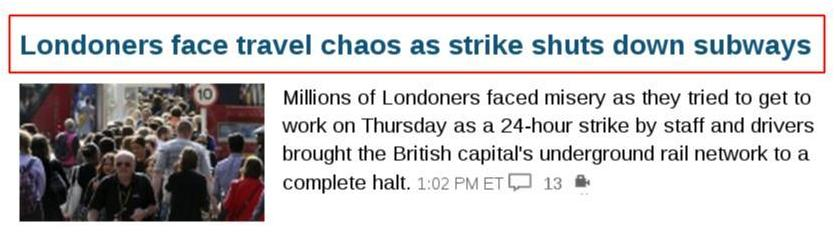
\includegraphics[width=\textwidth, height=4.5cm]{abstractive}
\caption{Example of abstractive summarization.}
\label{fig:abstractive}
\end{figure}

The limits of extractive summarization have been studied by \cite{he2000comparing}. They compare user preferences for various types of summaries of an audio-visual presentation. They demonstrate that the most preferred method of summarization is highlights and notes provided by the author, rather than transcripts or slides from the presentation. \cite{conroy2006topic} computed an oracle ROUGE score to investigate the same issue of the limits of extraction for news text. The oracle score is based on the maximum likelihood probability of words occurring in model summaries and is in turn used to generate summaries that perform better than any extracted and also human-generated summaries.

\subsection{ROUGE: Evaluation measure for Text Summarization}

ROUGE is an evaluation measure popularly used for evaluating quality of summaries and was proposed by \cite{lin-2004}. It measures the quality of the summary by comparing the output of the system being tested against a set of gold standard summaries. The intuition is that if the generated summary has enough in common with a set of human-written summaries, then it can be judged as a good summary. The different types of comparisons calculated are the unigram, bigram, trigram and least common subsequence(ROUGE-1,2,3 and L respectively). A set of gold standard summaries are used to encompass the number of possibilities while generating summaries. 

\begin{equation}
ROUGE-N = \frac{\sum\limits_{S \in \{Reference Summaries\}} \sum\limits_{gram_n \in S} Count_{match}(gram_n)}{\sum\limits_{S \in \{Reference Summaries\}} \sum\limits_{gram_n \in S} Count(gram_n)}
\end{equation}

The equation as described by \cite{lin2004looking} shows the calculation of the ROUGE-N score, where $n$ is the length of the n-gram, and $Count_{match}$ is the length of the matched n-grams in the summary and the reference summaries.

The use of multiple gold standard summaries gives rise to a subjective evaluation metric where the quality of the evaluation is dependent on the quality and number of the gold standard summaries. ROUGE also does not calculate take into account whether the summary is fluent or coherent. However, it is useful in the extractive text summarization systems where content retention needs to be judged since it uses n-gram co-occurrence statistics.

% \section{Stylistics}
%\change{remove this and put it in the formality part}
% Stylistics is referred to the characteristics of text that can be extracted from it that do not relate to the meaning of the text. Common examples of these include textual statistics such as length of sentences and words, parts of speech, function words etc. and finds applications in authorship attribution, semantic analysis, personality typing and so on. Studies on building lexicons for formality have been conducted and are discussed further later \chapref{chap:analysis}.

\section{Studies based on Twitter data}

There have been studies on a number of different issues related to Twitter data, including classifying tweets and sentiment analysis of tweets. \cite{ghosh2011entropy} classified the retweeting activity of users based on time intervals between retweets of a single user and frequency of retweets from unique users. 'Retweet' here means the occurrence of the same URL in a different tweet. The study was able to classify the retweeting as automatic or robotic retweeting, campaigns, news, blogs and so on, based on the time-interval and user-frequency distributions. In another study, \cite{chen2012extracting} were able to extract sentiment expressions from a corpus of tweets including both formal words and informal slang that bear sentiment.

Other studies using Twitter data include \cite{o2010tweetmotif}, who use topic summarization for a given search for better browsing. \cite{chakrabarti2011event} generate an event summary by learning about the event using a Hidden Markov Model over the tweets describing it. \cite{wang2014socially} generate a coherent event summary by treating summarization as an optimization problem for topic cohesion. \cite{inouye2011comparing} compare multiple summarization techniques to generate a summary of multi-post blogs on Twitter. \cite{wei2014utilizing} use tweets to help in generating better summaries of news articles.

% detailed analysis of this paper
As described in \chapref{chap:intro}, we analyze tweet generation using measures inspired by extractive summarization evaluation. There has been one study comparing different text summarization techniques for tweet generation by \cite{lloret2013towards}. Summarization systems were used to generate sentences lesser than 140 characters in length by summarizing documents, which could then be taken to be tweets. The system-generated tweets were evaluated using ROUGE measures \cite{lin2004rouge}. The ROUGE-1, ROUGE-2 and ROUGE-L measures were used, and a human-written reference tweet was taken to be the gold standard. %ROUGE has been known to work better when multiple reference summaries are used and is not meant to be used at the sentence level. This study uses ROUGE with a single reference summary, which is the reference tweet. However, given the size of a tweet, it can be argued that while generating a reference tweet from a single document, it is difficult to generate multiple reference tweets with largely varying content. \unsure{Is this reasoning okay?}

These studies show that extractive summarization algorithms may not generate good quality summaries despite giving high ROUGE evaluation scores. \cite{cheung2013towards} show that for the news genre, extractive summarization systems that are optimized for \textit{centrality}---that is, getting the core parts of the text into the summary---cannot perform well when compared to model summaries, since the model summaries are abstracted from the document to a large extent.
